% Options for packages loaded elsewhere
\PassOptionsToPackage{unicode}{hyperref}
\PassOptionsToPackage{hyphens}{url}
\PassOptionsToPackage{dvipsnames,svgnames,x11names}{xcolor}
%
\documentclass[
  letterpaper,
  DIV=11,
  numbers=noendperiod]{scrreprt}

\usepackage{amsmath,amssymb}
\usepackage{iftex}
\ifPDFTeX
  \usepackage[T1]{fontenc}
  \usepackage[utf8]{inputenc}
  \usepackage{textcomp} % provide euro and other symbols
\else % if luatex or xetex
  \usepackage{unicode-math}
  \defaultfontfeatures{Scale=MatchLowercase}
  \defaultfontfeatures[\rmfamily]{Ligatures=TeX,Scale=1}
\fi
\usepackage{lmodern}
\ifPDFTeX\else  
    % xetex/luatex font selection
\fi
% Use upquote if available, for straight quotes in verbatim environments
\IfFileExists{upquote.sty}{\usepackage{upquote}}{}
\IfFileExists{microtype.sty}{% use microtype if available
  \usepackage[]{microtype}
  \UseMicrotypeSet[protrusion]{basicmath} % disable protrusion for tt fonts
}{}
\makeatletter
\@ifundefined{KOMAClassName}{% if non-KOMA class
  \IfFileExists{parskip.sty}{%
    \usepackage{parskip}
  }{% else
    \setlength{\parindent}{0pt}
    \setlength{\parskip}{6pt plus 2pt minus 1pt}}
}{% if KOMA class
  \KOMAoptions{parskip=half}}
\makeatother
\usepackage{xcolor}
\setlength{\emergencystretch}{3em} % prevent overfull lines
\setcounter{secnumdepth}{5}
% Make \paragraph and \subparagraph free-standing
\makeatletter
\ifx\paragraph\undefined\else
  \let\oldparagraph\paragraph
  \renewcommand{\paragraph}{
    \@ifstar
      \xxxParagraphStar
      \xxxParagraphNoStar
  }
  \newcommand{\xxxParagraphStar}[1]{\oldparagraph*{#1}\mbox{}}
  \newcommand{\xxxParagraphNoStar}[1]{\oldparagraph{#1}\mbox{}}
\fi
\ifx\subparagraph\undefined\else
  \let\oldsubparagraph\subparagraph
  \renewcommand{\subparagraph}{
    \@ifstar
      \xxxSubParagraphStar
      \xxxSubParagraphNoStar
  }
  \newcommand{\xxxSubParagraphStar}[1]{\oldsubparagraph*{#1}\mbox{}}
  \newcommand{\xxxSubParagraphNoStar}[1]{\oldsubparagraph{#1}\mbox{}}
\fi
\makeatother

\usepackage{color}
\usepackage{fancyvrb}
\newcommand{\VerbBar}{|}
\newcommand{\VERB}{\Verb[commandchars=\\\{\}]}
\DefineVerbatimEnvironment{Highlighting}{Verbatim}{commandchars=\\\{\}}
% Add ',fontsize=\small' for more characters per line
\usepackage{framed}
\definecolor{shadecolor}{RGB}{241,243,245}
\newenvironment{Shaded}{\begin{snugshade}}{\end{snugshade}}
\newcommand{\AlertTok}[1]{\textcolor[rgb]{0.68,0.00,0.00}{#1}}
\newcommand{\AnnotationTok}[1]{\textcolor[rgb]{0.37,0.37,0.37}{#1}}
\newcommand{\AttributeTok}[1]{\textcolor[rgb]{0.40,0.45,0.13}{#1}}
\newcommand{\BaseNTok}[1]{\textcolor[rgb]{0.68,0.00,0.00}{#1}}
\newcommand{\BuiltInTok}[1]{\textcolor[rgb]{0.00,0.23,0.31}{#1}}
\newcommand{\CharTok}[1]{\textcolor[rgb]{0.13,0.47,0.30}{#1}}
\newcommand{\CommentTok}[1]{\textcolor[rgb]{0.37,0.37,0.37}{#1}}
\newcommand{\CommentVarTok}[1]{\textcolor[rgb]{0.37,0.37,0.37}{\textit{#1}}}
\newcommand{\ConstantTok}[1]{\textcolor[rgb]{0.56,0.35,0.01}{#1}}
\newcommand{\ControlFlowTok}[1]{\textcolor[rgb]{0.00,0.23,0.31}{\textbf{#1}}}
\newcommand{\DataTypeTok}[1]{\textcolor[rgb]{0.68,0.00,0.00}{#1}}
\newcommand{\DecValTok}[1]{\textcolor[rgb]{0.68,0.00,0.00}{#1}}
\newcommand{\DocumentationTok}[1]{\textcolor[rgb]{0.37,0.37,0.37}{\textit{#1}}}
\newcommand{\ErrorTok}[1]{\textcolor[rgb]{0.68,0.00,0.00}{#1}}
\newcommand{\ExtensionTok}[1]{\textcolor[rgb]{0.00,0.23,0.31}{#1}}
\newcommand{\FloatTok}[1]{\textcolor[rgb]{0.68,0.00,0.00}{#1}}
\newcommand{\FunctionTok}[1]{\textcolor[rgb]{0.28,0.35,0.67}{#1}}
\newcommand{\ImportTok}[1]{\textcolor[rgb]{0.00,0.46,0.62}{#1}}
\newcommand{\InformationTok}[1]{\textcolor[rgb]{0.37,0.37,0.37}{#1}}
\newcommand{\KeywordTok}[1]{\textcolor[rgb]{0.00,0.23,0.31}{\textbf{#1}}}
\newcommand{\NormalTok}[1]{\textcolor[rgb]{0.00,0.23,0.31}{#1}}
\newcommand{\OperatorTok}[1]{\textcolor[rgb]{0.37,0.37,0.37}{#1}}
\newcommand{\OtherTok}[1]{\textcolor[rgb]{0.00,0.23,0.31}{#1}}
\newcommand{\PreprocessorTok}[1]{\textcolor[rgb]{0.68,0.00,0.00}{#1}}
\newcommand{\RegionMarkerTok}[1]{\textcolor[rgb]{0.00,0.23,0.31}{#1}}
\newcommand{\SpecialCharTok}[1]{\textcolor[rgb]{0.37,0.37,0.37}{#1}}
\newcommand{\SpecialStringTok}[1]{\textcolor[rgb]{0.13,0.47,0.30}{#1}}
\newcommand{\StringTok}[1]{\textcolor[rgb]{0.13,0.47,0.30}{#1}}
\newcommand{\VariableTok}[1]{\textcolor[rgb]{0.07,0.07,0.07}{#1}}
\newcommand{\VerbatimStringTok}[1]{\textcolor[rgb]{0.13,0.47,0.30}{#1}}
\newcommand{\WarningTok}[1]{\textcolor[rgb]{0.37,0.37,0.37}{\textit{#1}}}

\providecommand{\tightlist}{%
  \setlength{\itemsep}{0pt}\setlength{\parskip}{0pt}}\usepackage{longtable,booktabs,array}
\usepackage{calc} % for calculating minipage widths
% Correct order of tables after \paragraph or \subparagraph
\usepackage{etoolbox}
\makeatletter
\patchcmd\longtable{\par}{\if@noskipsec\mbox{}\fi\par}{}{}
\makeatother
% Allow footnotes in longtable head/foot
\IfFileExists{footnotehyper.sty}{\usepackage{footnotehyper}}{\usepackage{footnote}}
\makesavenoteenv{longtable}
\usepackage{graphicx}
\makeatletter
\def\maxwidth{\ifdim\Gin@nat@width>\linewidth\linewidth\else\Gin@nat@width\fi}
\def\maxheight{\ifdim\Gin@nat@height>\textheight\textheight\else\Gin@nat@height\fi}
\makeatother
% Scale images if necessary, so that they will not overflow the page
% margins by default, and it is still possible to overwrite the defaults
% using explicit options in \includegraphics[width, height, ...]{}
\setkeys{Gin}{width=\maxwidth,height=\maxheight,keepaspectratio}
% Set default figure placement to htbp
\makeatletter
\def\fps@figure{htbp}
\makeatother
% definitions for citeproc citations
\NewDocumentCommand\citeproctext{}{}
\NewDocumentCommand\citeproc{mm}{%
  \begingroup\def\citeproctext{#2}\cite{#1}\endgroup}
\makeatletter
 % allow citations to break across lines
 \let\@cite@ofmt\@firstofone
 % avoid brackets around text for \cite:
 \def\@biblabel#1{}
 \def\@cite#1#2{{#1\if@tempswa , #2\fi}}
\makeatother
\newlength{\cslhangindent}
\setlength{\cslhangindent}{1.5em}
\newlength{\csllabelwidth}
\setlength{\csllabelwidth}{3em}
\newenvironment{CSLReferences}[2] % #1 hanging-indent, #2 entry-spacing
 {\begin{list}{}{%
  \setlength{\itemindent}{0pt}
  \setlength{\leftmargin}{0pt}
  \setlength{\parsep}{0pt}
  % turn on hanging indent if param 1 is 1
  \ifodd #1
   \setlength{\leftmargin}{\cslhangindent}
   \setlength{\itemindent}{-1\cslhangindent}
  \fi
  % set entry spacing
  \setlength{\itemsep}{#2\baselineskip}}}
 {\end{list}}
\usepackage{calc}
\newcommand{\CSLBlock}[1]{\hfill\break\parbox[t]{\linewidth}{\strut\ignorespaces#1\strut}}
\newcommand{\CSLLeftMargin}[1]{\parbox[t]{\csllabelwidth}{\strut#1\strut}}
\newcommand{\CSLRightInline}[1]{\parbox[t]{\linewidth - \csllabelwidth}{\strut#1\strut}}
\newcommand{\CSLIndent}[1]{\hspace{\cslhangindent}#1}

\KOMAoption{captions}{tableheading}
\makeatletter
\@ifpackageloaded{bookmark}{}{\usepackage{bookmark}}
\makeatother
\makeatletter
\@ifpackageloaded{caption}{}{\usepackage{caption}}
\AtBeginDocument{%
\ifdefined\contentsname
  \renewcommand*\contentsname{Table of contents}
\else
  \newcommand\contentsname{Table of contents}
\fi
\ifdefined\listfigurename
  \renewcommand*\listfigurename{List of Figures}
\else
  \newcommand\listfigurename{List of Figures}
\fi
\ifdefined\listtablename
  \renewcommand*\listtablename{List of Tables}
\else
  \newcommand\listtablename{List of Tables}
\fi
\ifdefined\figurename
  \renewcommand*\figurename{Figure}
\else
  \newcommand\figurename{Figure}
\fi
\ifdefined\tablename
  \renewcommand*\tablename{Table}
\else
  \newcommand\tablename{Table}
\fi
}
\@ifpackageloaded{float}{}{\usepackage{float}}
\floatstyle{ruled}
\@ifundefined{c@chapter}{\newfloat{codelisting}{h}{lop}}{\newfloat{codelisting}{h}{lop}[chapter]}
\floatname{codelisting}{Listing}
\newcommand*\listoflistings{\listof{codelisting}{List of Listings}}
\makeatother
\makeatletter
\makeatother
\makeatletter
\@ifpackageloaded{caption}{}{\usepackage{caption}}
\@ifpackageloaded{subcaption}{}{\usepackage{subcaption}}
\makeatother

\ifLuaTeX
  \usepackage{selnolig}  % disable illegal ligatures
\fi
\usepackage{bookmark}

\IfFileExists{xurl.sty}{\usepackage{xurl}}{} % add URL line breaks if available
\urlstyle{same} % disable monospaced font for URLs
\hypersetup{
  pdftitle={Structural equation modeling with lavaan in R: Examples and excercises},
  pdfauthor={Deon de Bruin},
  colorlinks=true,
  linkcolor={blue},
  filecolor={Maroon},
  citecolor={Blue},
  urlcolor={Blue},
  pdfcreator={LaTeX via pandoc}}


\title{Structural equation modeling with lavaan in R: Examples and
excercises}
\author{Deon de Bruin}
\date{2025-01-20}

\begin{document}
\maketitle

\renewcommand*\contentsname{Table of contents}
{
\hypersetup{linkcolor=}
\setcounter{tocdepth}{2}
\tableofcontents
}

\bookmarksetup{startatroot}

\chapter*{Preface}\label{preface}
\addcontentsline{toc}{chapter}{Preface}

\markboth{Preface}{Preface}

This is a Quarto book.

To learn more about Quarto books visit
\url{https://quarto.org/docs/books}.

\begin{Shaded}
\begin{Highlighting}[]
\DecValTok{1} \SpecialCharTok{+} \DecValTok{1}
\end{Highlighting}
\end{Shaded}

\begin{verbatim}
[1] 2
\end{verbatim}

\bookmarksetup{startatroot}

\chapter{Introduction}\label{introduction}

This is a book created from markdown and executable code.

See Knuth (1984) for additional discussion of literate programming.

\begin{Shaded}
\begin{Highlighting}[]
\DecValTok{1} \SpecialCharTok{+} \DecValTok{1}
\end{Highlighting}
\end{Shaded}

\begin{verbatim}
[1] 2
\end{verbatim}

\part{Part I: Measurement model}

\bookmarksetup{startatroot}

\chapter{Single factor model}\label{single-factor-model}

\begin{Shaded}
\begin{Highlighting}[]
\FunctionTok{library}\NormalTok{(psychTools)}
\FunctionTok{library}\NormalTok{(lavaan)}
\FunctionTok{library}\NormalTok{(flexplavaan)}

\NormalTok{mod1 }\OtherTok{\textless{}{-}} \StringTok{\textquotesingle{}}
\StringTok{Agreeableness =\textasciitilde{} A1 + A2 + A3 + A4 + A5}
\StringTok{\textquotesingle{}}

\NormalTok{fit.mod1 }\OtherTok{\textless{}{-}} \FunctionTok{cfa}\NormalTok{(mod1, }\AttributeTok{data =}\NormalTok{ bfi)}
\FunctionTok{summary}\NormalTok{(fit.mod1, }\AttributeTok{standardized =} \ConstantTok{TRUE}\NormalTok{, }\AttributeTok{fit.measures =} \ConstantTok{TRUE}\NormalTok{)}
\end{Highlighting}
\end{Shaded}

\begin{verbatim}
lavaan 0.6-19 ended normally after 33 iterations

  Estimator                                         ML
  Optimization method                           NLMINB
  Number of model parameters                        10

                                                  Used       Total
  Number of observations                          2709        2800

Model Test User Model:
                                                      
  Test statistic                                86.696
  Degrees of freedom                                 5
  P-value (Chi-square)                           0.000

Model Test Baseline Model:

  Test statistic                              2533.636
  Degrees of freedom                                10
  P-value                                        0.000

User Model versus Baseline Model:

  Comparative Fit Index (CFI)                    0.968
  Tucker-Lewis Index (TLI)                       0.935

Loglikelihood and Information Criteria:

  Loglikelihood user model (H0)             -21777.580
  Loglikelihood unrestricted model (H1)     -21734.232
                                                      
  Akaike (AIC)                               43575.160
  Bayesian (BIC)                             43634.203
  Sample-size adjusted Bayesian (SABIC)      43602.430

Root Mean Square Error of Approximation:

  RMSEA                                          0.078
  90 Percent confidence interval - lower         0.064
  90 Percent confidence interval - upper         0.092
  P-value H_0: RMSEA <= 0.050                    0.001
  P-value H_0: RMSEA >= 0.080                    0.415

Standardized Root Mean Square Residual:

  SRMR                                           0.032

Parameter Estimates:

  Standard errors                             Standard
  Information                                 Expected
  Information saturated (h1) model          Structured

Latent Variables:
                   Estimate  Std.Err  z-value  P(>|z|)   Std.lv  Std.all
  Agreeableness =~                                                      
    A1                1.000                               0.528    0.376
    A2               -1.465    0.090  -16.310    0.000   -0.774   -0.658
    A3               -1.880    0.113  -16.696    0.000   -0.994   -0.762
    A4               -1.358    0.093  -14.626    0.000   -0.717   -0.483
    A5               -1.497    0.093  -16.098    0.000   -0.791   -0.627

Variances:
                   Estimate  Std.Err  z-value  P(>|z|)   Std.lv  Std.all
   .A1                1.693    0.048   34.915    0.000    1.693    0.858
   .A2                0.784    0.029   27.443    0.000    0.784    0.567
   .A3                0.714    0.035   20.314    0.000    0.714    0.420
   .A4                1.694    0.051   33.277    0.000    1.694    0.767
   .A5                0.965    0.033   28.977    0.000    0.965    0.607
    Agreeableness     0.279    0.031    8.870    0.000    1.000    1.000
\end{verbatim}

\begin{Shaded}
\begin{Highlighting}[]
\FunctionTok{visualize}\NormalTok{(fit.mod1)}
\end{Highlighting}
\end{Shaded}

\includegraphics{Spearman_files/figure-pdf/unnamed-chunk-1-1.pdf}

\begin{Shaded}
\begin{Highlighting}[]
\FunctionTok{measurement\_plot}\NormalTok{(fit.mod1, }\AttributeTok{sample =} \DecValTok{300}\NormalTok{)}
\end{Highlighting}
\end{Shaded}

\includegraphics{Spearman_files/figure-pdf/unnamed-chunk-1-2.pdf}

\begin{Shaded}
\begin{Highlighting}[]
\FunctionTok{residual\_plots}\NormalTok{(fit.mod1)}
\end{Highlighting}
\end{Shaded}

\includegraphics{Spearman_files/figure-pdf/unnamed-chunk-1-3.pdf}

\begin{Shaded}
\begin{Highlighting}[]
\NormalTok{GWS2020 }\OtherTok{\textless{}{-}} \FunctionTok{read.csv}\NormalTok{(}\StringTok{"C:/Users/deondb/Downloads/GWS2020.csv"}\NormalTok{)}

\NormalTok{modgws }\OtherTok{\textless{}{-}} \StringTok{\textquotesingle{}}
\StringTok{Stress =\textasciitilde{} Item1 + Item2 + Item3 + Item4 + Item5 + Item6 + Item7 + Item8 + Item9}
\StringTok{\textquotesingle{}}

\NormalTok{fit.modgws }\OtherTok{\textless{}{-}} \FunctionTok{cfa}\NormalTok{(modgws, }\AttributeTok{data =}\NormalTok{ GWS2020)}
\FunctionTok{summary}\NormalTok{(fit.modgws, }\AttributeTok{standardized =} \ConstantTok{TRUE}\NormalTok{, }\AttributeTok{fit.measures =} \ConstantTok{TRUE}\NormalTok{)}
\end{Highlighting}
\end{Shaded}

\begin{verbatim}
lavaan 0.6-19 ended normally after 22 iterations

  Estimator                                         ML
  Optimization method                           NLMINB
  Number of model parameters                        18

  Number of observations                          1377

Model Test User Model:
                                                      
  Test statistic                               808.572
  Degrees of freedom                                27
  P-value (Chi-square)                           0.000

Model Test Baseline Model:

  Test statistic                              6506.495
  Degrees of freedom                                36
  P-value                                        0.000

User Model versus Baseline Model:

  Comparative Fit Index (CFI)                    0.879
  Tucker-Lewis Index (TLI)                       0.839

Loglikelihood and Information Criteria:

  Loglikelihood user model (H0)             -14826.170
  Loglikelihood unrestricted model (H1)     -14421.884
                                                      
  Akaike (AIC)                               29688.341
  Bayesian (BIC)                             29782.439
  Sample-size adjusted Bayesian (SABIC)      29725.260

Root Mean Square Error of Approximation:

  RMSEA                                          0.145
  90 Percent confidence interval - lower         0.136
  90 Percent confidence interval - upper         0.154
  P-value H_0: RMSEA <= 0.050                    0.000
  P-value H_0: RMSEA >= 0.080                    1.000

Standardized Root Mean Square Residual:

  SRMR                                           0.057

Parameter Estimates:

  Standard errors                             Standard
  Information                                 Expected
  Information saturated (h1) model          Structured

Latent Variables:
                   Estimate  Std.Err  z-value  P(>|z|)   Std.lv  Std.all
  Stress =~                                                             
    Item1             1.000                               0.810    0.762
    Item2             1.114    0.036   31.162    0.000    0.902    0.814
    Item3             0.963    0.035   27.841    0.000    0.780    0.737
    Item4             0.895    0.036   24.948    0.000    0.725    0.668
    Item5             0.763    0.031   24.824    0.000    0.618    0.665
    Item6             0.831    0.029   28.328    0.000    0.673    0.748
    Item7             0.813    0.035   23.238    0.000    0.659    0.627
    Item8             0.837    0.031   27.235    0.000    0.678    0.723
    Item9             0.771    0.032   24.225    0.000    0.624    0.651

Variances:
                   Estimate  Std.Err  z-value  P(>|z|)   Std.lv  Std.all
   .Item1             0.474    0.021   22.527    0.000    0.474    0.419
   .Item2             0.414    0.020   20.962    0.000    0.414    0.337
   .Item3             0.511    0.022   23.054    0.000    0.511    0.457
   .Item4             0.651    0.027   24.084    0.000    0.651    0.553
   .Item5             0.481    0.020   24.118    0.000    0.481    0.557
   .Item6             0.356    0.016   22.826    0.000    0.356    0.440
   .Item7             0.671    0.027   24.515    0.000    0.671    0.607
   .Item8             0.420    0.018   23.311    0.000    0.420    0.478
   .Item9             0.530    0.022   24.278    0.000    0.530    0.576
    Stress            0.656    0.041   16.177    0.000    1.000    1.000
\end{verbatim}

\begin{Shaded}
\begin{Highlighting}[]
\FunctionTok{visualize}\NormalTok{(fit.modgws, }\AttributeTok{subset =} \DecValTok{1}\SpecialCharTok{:}\DecValTok{9}\NormalTok{)}
\end{Highlighting}
\end{Shaded}

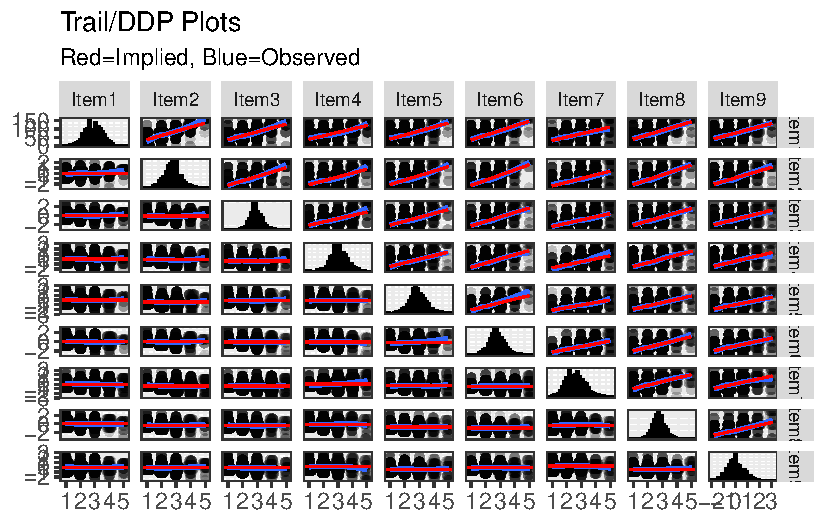
\includegraphics{Spearman_files/figure-pdf/unnamed-chunk-2-1.pdf}

\begin{Shaded}
\begin{Highlighting}[]
\FunctionTok{measurement\_plot}\NormalTok{(fit.modgws, }\AttributeTok{sample =} \DecValTok{300}\NormalTok{)}
\end{Highlighting}
\end{Shaded}

\includegraphics{Spearman_files/figure-pdf/unnamed-chunk-2-2.pdf}

\begin{Shaded}
\begin{Highlighting}[]
\FunctionTok{residual\_plots}\NormalTok{(fit.modgws)}
\end{Highlighting}
\end{Shaded}

\includegraphics{Spearman_files/figure-pdf/unnamed-chunk-2-3.pdf}

\bookmarksetup{startatroot}

\chapter{Multiple factors}\label{multiple-factors}

\begin{Shaded}
\begin{Highlighting}[]
\FunctionTok{library}\NormalTok{(lavaan)}
\FunctionTok{library}\NormalTok{(flexplavaan)}
\FunctionTok{library}\NormalTok{(psychTools)}


\NormalTok{mod3 }\OtherTok{\textless{}{-}} \StringTok{\textquotesingle{}}
\StringTok{Neuroticism   =\textasciitilde{} N1 + N2 + N3 + N4 + N5}
\StringTok{Agreeableness =\textasciitilde{} A1 + A2 + A3 + A4 + A5}

\StringTok{N1 \textasciitilde{}\textasciitilde{} N2}
\StringTok{\textquotesingle{}}

\NormalTok{fit.mod3 }\OtherTok{\textless{}{-}} \FunctionTok{cfa}\NormalTok{(}\AttributeTok{model =}\NormalTok{ mod3, }
                \AttributeTok{data  =}\NormalTok{ bfi)}

\FunctionTok{summary}\NormalTok{(fit.mod3, }
        \AttributeTok{standardized =} \ConstantTok{TRUE}\NormalTok{, }
        \AttributeTok{fit.measures =} \ConstantTok{TRUE}\NormalTok{)}
\end{Highlighting}
\end{Shaded}

\begin{verbatim}
lavaan 0.6-19 ended normally after 39 iterations

  Estimator                                         ML
  Optimization method                           NLMINB
  Number of model parameters                        22

                                                  Used       Total
  Number of observations                          2618        2800

Model Test User Model:
                                                      
  Test statistic                               394.745
  Degrees of freedom                                33
  P-value (Chi-square)                           0.000

Model Test Baseline Model:

  Test statistic                              7465.706
  Degrees of freedom                                45
  P-value                                        0.000

User Model versus Baseline Model:

  Comparative Fit Index (CFI)                    0.951
  Tucker-Lewis Index (TLI)                       0.934

Loglikelihood and Information Criteria:

  Loglikelihood user model (H0)             -43229.863
  Loglikelihood unrestricted model (H1)     -43032.491
                                                      
  Akaike (AIC)                               86503.726
  Bayesian (BIC)                             86632.870
  Sample-size adjusted Bayesian (SABIC)      86562.969

Root Mean Square Error of Approximation:

  RMSEA                                          0.065
  90 Percent confidence interval - lower         0.059
  90 Percent confidence interval - upper         0.071
  P-value H_0: RMSEA <= 0.050                    0.000
  P-value H_0: RMSEA >= 0.080                    0.000

Standardized Root Mean Square Residual:

  SRMR                                           0.048

Parameter Estimates:

  Standard errors                             Standard
  Information                                 Expected
  Information saturated (h1) model          Structured

Latent Variables:
                   Estimate  Std.Err  z-value  P(>|z|)   Std.lv  Std.all
  Neuroticism =~                                                        
    N1                1.000                               1.069    0.681
    N2                0.940    0.024   38.841    0.000    1.005    0.658
    N3                1.206    0.041   29.617    0.000    1.289    0.807
    N4                0.944    0.035   26.800    0.000    1.009    0.643
    N5                0.833    0.035   23.538    0.000    0.890    0.549
  Agreeableness =~                                                      
    A1                1.000                               0.542    0.387
    A2               -1.413    0.086  -16.450    0.000   -0.765   -0.651
    A3               -1.838    0.109  -16.933    0.000   -0.996   -0.761
    A4               -1.343    0.091  -14.789    0.000   -0.728   -0.488
    A5               -1.487    0.091  -16.357    0.000   -0.806   -0.638

Covariances:
                   Estimate  Std.Err  z-value  P(>|z|)   Std.lv  Std.all
 .N1 ~~                                                                 
   .N2                0.621    0.040   15.696    0.000    0.621    0.471
  Neuroticism ~~                                                        
    Agreeableness     0.117    0.016    7.304    0.000    0.203    0.203

Variances:
                   Estimate  Std.Err  z-value  P(>|z|)   Std.lv  Std.all
   .N1                1.319    0.048   27.230    0.000    1.319    0.536
   .N2                1.319    0.047   28.112    0.000    1.319    0.567
   .N3                0.890    0.048   18.678    0.000    0.890    0.349
   .N4                1.447    0.049   29.606    0.000    1.447    0.587
   .N5                1.836    0.057   32.264    0.000    1.836    0.699
   .A1                1.668    0.049   34.239    0.000    1.668    0.850
   .A2                0.795    0.029   27.568    0.000    0.795    0.576
   .A3                0.719    0.035   20.374    0.000    0.719    0.420
   .A4                1.692    0.052   32.681    0.000    1.692    0.762
   .A5                0.943    0.033   28.181    0.000    0.943    0.592
    Neuroticism       1.142    0.066   17.384    0.000    1.000    1.000
    Agreeableness     0.293    0.033    9.006    0.000    1.000    1.000
\end{verbatim}

\begin{Shaded}
\begin{Highlighting}[]
\FunctionTok{visualize}\NormalTok{(fit.mod3, }
          \AttributeTok{subset =} \DecValTok{1}\SpecialCharTok{:}\DecValTok{10}\NormalTok{)}
\end{Highlighting}
\end{Shaded}

\includegraphics{Multiple_factors_files/figure-pdf/unnamed-chunk-1-1.pdf}

\begin{Shaded}
\begin{Highlighting}[]
\FunctionTok{measurement\_plot}\NormalTok{(fit.mod3, }
                 \AttributeTok{sample =} \DecValTok{300}\NormalTok{)}
\end{Highlighting}
\end{Shaded}

\begin{verbatim}
$Neuroticism
\end{verbatim}

\includegraphics{Multiple_factors_files/figure-pdf/unnamed-chunk-1-2.pdf}

\begin{verbatim}

$Agreeableness
\end{verbatim}

\includegraphics{Multiple_factors_files/figure-pdf/unnamed-chunk-1-3.pdf}

\begin{Shaded}
\begin{Highlighting}[]
\FunctionTok{residual\_plots}\NormalTok{(fit.mod3)}
\end{Highlighting}
\end{Shaded}

\includegraphics{Multiple_factors_files/figure-pdf/unnamed-chunk-1-4.pdf}

\part{Part II: Diagnosing and improving the measurement model}

\bookmarksetup{startatroot}

\chapter{Modification Indices}\label{modification-indices}

\begin{Shaded}
\begin{Highlighting}[]
\FunctionTok{library}\NormalTok{(lavaan)}
\end{Highlighting}
\end{Shaded}

\begin{verbatim}
This is lavaan 0.6-19
lavaan is FREE software! Please report any bugs.
\end{verbatim}

\begin{Shaded}
\begin{Highlighting}[]
\FunctionTok{library}\NormalTok{(psychTools)}
\NormalTok{mod3 }\OtherTok{\textless{}{-}} \StringTok{\textquotesingle{}}
\StringTok{Neuroticism   =\textasciitilde{} N1 + N2 + N3 + N4 + N5}
\StringTok{Agreeableness =\textasciitilde{} A1 + A2 + A3 + A4 + A5}
\StringTok{\textquotesingle{}}

\NormalTok{fit.mod3 }\OtherTok{\textless{}{-}} \FunctionTok{cfa}\NormalTok{(}\AttributeTok{model =}\NormalTok{ mod3, }
                \AttributeTok{data  =}\NormalTok{ bfi)}

\FunctionTok{summary}\NormalTok{(fit.mod3, }
        \AttributeTok{standardized =} \ConstantTok{TRUE}\NormalTok{, }
        \AttributeTok{fit.measures =} \ConstantTok{TRUE}\NormalTok{)}
\end{Highlighting}
\end{Shaded}

\begin{verbatim}
lavaan 0.6-19 ended normally after 36 iterations

  Estimator                                         ML
  Optimization method                           NLMINB
  Number of model parameters                        21

                                                  Used       Total
  Number of observations                          2618        2800

Model Test User Model:
                                                      
  Test statistic                               694.620
  Degrees of freedom                                34
  P-value (Chi-square)                           0.000

Model Test Baseline Model:

  Test statistic                              7465.706
  Degrees of freedom                                45
  P-value                                        0.000

User Model versus Baseline Model:

  Comparative Fit Index (CFI)                    0.911
  Tucker-Lewis Index (TLI)                       0.882

Loglikelihood and Information Criteria:

  Loglikelihood user model (H0)             -43379.800
  Loglikelihood unrestricted model (H1)     -43032.491
                                                      
  Akaike (AIC)                               86801.601
  Bayesian (BIC)                             86924.874
  Sample-size adjusted Bayesian (SABIC)      86858.151

Root Mean Square Error of Approximation:

  RMSEA                                          0.086
  90 Percent confidence interval - lower         0.081
  90 Percent confidence interval - upper         0.092
  P-value H_0: RMSEA <= 0.050                    0.000
  P-value H_0: RMSEA >= 0.080                    0.966

Standardized Root Mean Square Residual:

  SRMR                                           0.054

Parameter Estimates:

  Standard errors                             Standard
  Information                                 Expected
  Information saturated (h1) model          Structured

Latent Variables:
                   Estimate  Std.Err  z-value  P(>|z|)   Std.lv  Std.all
  Neuroticism =~                                                        
    N1                1.000                               1.292    0.823
    N2                0.949    0.023   40.791    0.000    1.226    0.803
    N3                0.884    0.024   36.571    0.000    1.141    0.714
    N4                0.680    0.024   27.853    0.000    0.878    0.559
    N5                0.626    0.025   24.591    0.000    0.809    0.499
  Agreeableness =~                                                      
    A1                1.000                               0.545    0.389
    A2               -1.404    0.085  -16.527    0.000   -0.765   -0.651
    A3               -1.822    0.107  -17.018    0.000   -0.992   -0.759
    A4               -1.338    0.090  -14.855    0.000   -0.729   -0.489
    A5               -1.483    0.090  -16.448    0.000   -0.808   -0.640

Covariances:
                   Estimate  Std.Err  z-value  P(>|z|)   Std.lv  Std.all
  Neuroticism ~~                                                        
    Agreeableness     0.155    0.019    8.049    0.000    0.220    0.220

Variances:
                   Estimate  Std.Err  z-value  P(>|z|)   Std.lv  Std.all
   .N1                0.793    0.036   22.094    0.000    0.793    0.322
   .N2                0.826    0.035   23.877    0.000    0.826    0.355
   .N3                1.249    0.043   29.352    0.000    1.249    0.490
   .N4                1.694    0.051   33.284    0.000    1.694    0.687
   .N5                1.974    0.058   34.081    0.000    1.974    0.751
   .A1                1.665    0.049   34.211    0.000    1.665    0.849
   .A2                0.796    0.029   27.597    0.000    0.796    0.576
   .A3                0.725    0.035   20.614    0.000    0.725    0.424
   .A4                1.690    0.052   32.667    0.000    1.690    0.761
   .A5                0.939    0.033   28.108    0.000    0.939    0.590
    Neuroticism       1.668    0.070   23.696    0.000    1.000    1.000
    Agreeableness     0.297    0.033    9.060    0.000    1.000    1.000
\end{verbatim}

\begin{Shaded}
\begin{Highlighting}[]
\FunctionTok{modificationindices}\NormalTok{(fit.mod3)}
\end{Highlighting}
\end{Shaded}

\begin{verbatim}
             lhs op rhs      mi    epc sepc.lv sepc.all sepc.nox
24   Neuroticism =~  A1  19.035  0.098   0.127    0.091    0.091
25   Neuroticism =~  A2  20.795  0.079   0.102    0.087    0.087
26   Neuroticism =~  A3  29.798  0.104   0.135    0.103    0.103
27   Neuroticism =~  A4   5.262 -0.053  -0.069   -0.046   -0.046
28   Neuroticism =~  A5  50.336 -0.132  -0.171   -0.135   -0.135
29 Agreeableness =~  N1   0.630  0.038   0.021    0.013    0.013
30 Agreeableness =~  N2   0.295  0.025   0.014    0.009    0.009
31 Agreeableness =~  N3  10.202 -0.168  -0.091   -0.057   -0.057
32 Agreeableness =~  N4  25.954  0.293   0.160    0.102    0.102
33 Agreeableness =~  N5  11.128 -0.205  -0.112   -0.069   -0.069
34            N1 ~~  N2 345.707  0.775   0.775    0.958    0.958
35            N1 ~~  N3  52.136 -0.272  -0.272   -0.274   -0.274
36            N1 ~~  N4  76.839 -0.291  -0.291   -0.251   -0.251
37            N1 ~~  N5  19.022 -0.149  -0.149   -0.119   -0.119
38            N1 ~~  A1  24.399  0.137   0.137    0.119    0.119
39            N1 ~~  A2   4.495 -0.044  -0.044   -0.055   -0.055
40            N1 ~~  A3  13.106  0.079   0.079    0.104    0.104
41            N1 ~~  A4   5.855  0.069   0.069    0.059    0.059
42            N1 ~~  A5   5.301 -0.051  -0.051   -0.059   -0.059
43            N2 ~~  N3  37.647 -0.220  -0.220   -0.216   -0.216
44            N2 ~~  N4  68.849 -0.266  -0.266   -0.225   -0.225
45            N2 ~~  N5  42.497 -0.217  -0.217   -0.170   -0.170
46            N2 ~~  A1   3.438  0.051   0.051    0.043    0.043
47            N2 ~~  A2  14.146  0.077   0.077    0.095    0.095
48            N2 ~~  A3   0.861  0.020   0.020    0.026    0.026
49            N2 ~~  A4  14.742 -0.108  -0.108   -0.091   -0.091
50            N2 ~~  A5   3.613 -0.042  -0.042   -0.048   -0.048
51            N3 ~~  N4 163.251  0.436   0.436    0.300    0.300
52            N3 ~~  N5  47.254  0.247   0.247    0.157    0.157
53            N3 ~~  A1   0.111  0.010   0.010    0.007    0.007
54            N3 ~~  A2   0.254  0.012   0.012    0.012    0.012
55            N3 ~~  A3   3.474  0.046   0.046    0.048    0.048
56            N3 ~~  A4   0.614  0.025   0.025    0.017    0.017
57            N3 ~~  A5   0.171  0.010   0.010    0.010    0.010
58            N4 ~~  N5  86.112  0.360   0.360    0.197    0.197
59            N4 ~~  A1  17.767 -0.146  -0.146   -0.087   -0.087
60            N4 ~~  A2   0.251  0.013   0.013    0.011    0.011
61            N4 ~~  A3   3.030 -0.047  -0.047   -0.043   -0.043
62            N4 ~~  A4  20.479 -0.161  -0.161   -0.095   -0.095
63            N4 ~~  A5  10.813 -0.092  -0.092   -0.073   -0.073
64            N5 ~~  A1   8.114 -0.106  -0.106   -0.058   -0.058
65            N5 ~~  A2   7.324  0.075   0.075    0.060    0.060
66            N5 ~~  A3   5.725 -0.069  -0.069   -0.058   -0.058
67            N5 ~~  A4   8.224  0.109   0.109    0.060    0.060
68            N5 ~~  A5   0.301  0.016   0.016    0.012    0.012
69            A1 ~~  A2  64.589 -0.219  -0.219   -0.190   -0.190
70            A1 ~~  A3   6.688  0.080   0.080    0.073    0.073
71            A1 ~~  A4   4.991  0.080   0.080    0.048    0.048
72            A1 ~~  A5  22.962  0.140   0.140    0.112    0.112
73            A2 ~~  A3   0.654 -0.027  -0.027   -0.036   -0.036
74            A2 ~~  A4   3.109  0.051   0.051    0.044    0.044
75            A2 ~~  A5  20.439 -0.124  -0.124   -0.143   -0.143
76            A3 ~~  A4   0.417 -0.022  -0.022   -0.020   -0.020
77            A3 ~~  A5  31.301  0.197   0.197    0.239    0.239
78            A4 ~~  A5   0.192 -0.014  -0.014   -0.011   -0.011
\end{verbatim}

\bookmarksetup{startatroot}

\chapter{Exploratory factor analysis}\label{exploratory-factor-analysis}

\begin{Shaded}
\begin{Highlighting}[]
\FunctionTok{library}\NormalTok{(lavaan)}
\FunctionTok{library}\NormalTok{(flexplavaan)}
\FunctionTok{library}\NormalTok{(psychTools)}
\FunctionTok{library}\NormalTok{(psych)}

\FunctionTok{scree}\NormalTok{(bfi[}\FunctionTok{c}\NormalTok{(}\DecValTok{1}\SpecialCharTok{:}\DecValTok{5}\NormalTok{, }\DecValTok{16}\SpecialCharTok{:}\DecValTok{20}\NormalTok{)])}
\end{Highlighting}
\end{Shaded}

\includegraphics{EFA_files/figure-pdf/unnamed-chunk-1-1.pdf}

\begin{Shaded}
\begin{Highlighting}[]
\FunctionTok{fa.parallel}\NormalTok{(bfi[}\FunctionTok{c}\NormalTok{(}\DecValTok{1}\SpecialCharTok{:}\DecValTok{5}\NormalTok{, }\DecValTok{16}\SpecialCharTok{:}\DecValTok{20}\NormalTok{)])}
\end{Highlighting}
\end{Shaded}

\includegraphics{EFA_files/figure-pdf/unnamed-chunk-1-2.pdf}

\begin{verbatim}
Parallel analysis suggests that the number of factors =  3  and the number of components =  2 
\end{verbatim}

\begin{Shaded}
\begin{Highlighting}[]
\FunctionTok{fa}\NormalTok{(bfi[}\FunctionTok{c}\NormalTok{(}\DecValTok{1}\SpecialCharTok{:}\DecValTok{5}\NormalTok{, }\DecValTok{16}\SpecialCharTok{:}\DecValTok{20}\NormalTok{)], }\AttributeTok{nfactors =} \DecValTok{2}\NormalTok{)}
\end{Highlighting}
\end{Shaded}

\begin{verbatim}
Factor Analysis using method =  minres
Call: fa(r = bfi[c(1:5, 16:20)], nfactors = 2)
Standardized loadings (pattern matrix) based upon correlation matrix
     MR1   MR2   h2   u2 com
A1  0.07 -0.36 0.14 0.86 1.1
A2  0.05  0.69 0.47 0.53 1.0
A3  0.03  0.76 0.56 0.44 1.0
A4 -0.05  0.47 0.24 0.76 1.0
A5 -0.12  0.60 0.39 0.61 1.1
N1  0.78 -0.03 0.61 0.39 1.0
N2  0.76 -0.02 0.58 0.42 1.0
N3  0.77  0.05 0.58 0.42 1.0
N4  0.58 -0.08 0.36 0.64 1.0
N5  0.54  0.08 0.29 0.71 1.0

                       MR1  MR2
SS loadings           2.44 1.78
Proportion Var        0.24 0.18
Cumulative Var        0.24 0.42
Proportion Explained  0.58 0.42
Cumulative Proportion 0.58 1.00

 With factor correlations of 
      MR1   MR2
MR1  1.00 -0.19
MR2 -0.19  1.00

Mean item complexity =  1
Test of the hypothesis that 2 factors are sufficient.

df null model =  45  with the objective function =  2.82 with Chi Square =  7880.99
df of  the model are 26  and the objective function was  0.23 

The root mean square of the residuals (RMSR) is  0.04 
The df corrected root mean square of the residuals is  0.05 

The harmonic n.obs is  2759 with the empirical chi square  396.78  with prob <  5.7e-68 
The total n.obs was  2800  with Likelihood Chi Square =  636.27  with prob <  1.6e-117 

Tucker Lewis Index of factoring reliability =  0.865
RMSEA index =  0.092  and the 90 % confidence intervals are  0.085 0.098
BIC =  429.9
Fit based upon off diagonal values = 0.98
Measures of factor score adequacy             
                                                   MR1  MR2
Correlation of (regression) scores with factors   0.92 0.88
Multiple R square of scores with factors          0.84 0.77
Minimum correlation of possible factor scores     0.68 0.54
\end{verbatim}

\begin{Shaded}
\begin{Highlighting}[]
\FunctionTok{fa}\NormalTok{(bfi[}\FunctionTok{c}\NormalTok{(}\DecValTok{1}\SpecialCharTok{:}\DecValTok{5}\NormalTok{, }\DecValTok{16}\SpecialCharTok{:}\DecValTok{20}\NormalTok{)], }\AttributeTok{nfactors =} \DecValTok{3}\NormalTok{)}
\end{Highlighting}
\end{Shaded}

\begin{verbatim}
Factor Analysis using method =  minres
Call: fa(r = bfi[c(1:5, 16:20)], nfactors = 3)
Standardized loadings (pattern matrix) based upon correlation matrix
     MR2   MR1   MR3   h2   u2 com
A1 -0.36  0.24 -0.17 0.17 0.83 2.2
A2  0.69 -0.04  0.09 0.47 0.53 1.0
A3  0.75  0.06 -0.05 0.57 0.43 1.0
A4  0.47  0.00 -0.07 0.24 0.76 1.0
A5  0.59 -0.05 -0.10 0.40 0.60 1.1
N1 -0.01  0.88 -0.02 0.76 0.24 1.0
N2 -0.01  0.77  0.05 0.65 0.35 1.0
N3  0.05  0.37  0.47 0.57 0.43 1.9
N4 -0.07 -0.02  0.75 0.57 0.43 1.0
N5  0.08  0.16  0.46 0.32 0.68 1.3

                       MR2  MR1  MR3
SS loadings           1.77 1.74 1.19
Proportion Var        0.18 0.17 0.12
Cumulative Var        0.18 0.35 0.47
Proportion Explained  0.38 0.37 0.25
Cumulative Proportion 0.38 0.75 1.00

 With factor correlations of 
      MR2   MR1   MR3
MR2  1.00 -0.16 -0.15
MR1 -0.16  1.00  0.63
MR3 -0.15  0.63  1.00

Mean item complexity =  1.3
Test of the hypothesis that 3 factors are sufficient.

df null model =  45  with the objective function =  2.82 with Chi Square =  7880.99
df of  the model are 18  and the objective function was  0.06 

The root mean square of the residuals (RMSR) is  0.02 
The df corrected root mean square of the residuals is  0.04 

The harmonic n.obs is  2759 with the empirical chi square  121.95  with prob <  1.8e-17 
The total n.obs was  2800  with Likelihood Chi Square =  176.12  with prob <  5.6e-28 

Tucker Lewis Index of factoring reliability =  0.95
RMSEA index =  0.056  and the 90 % confidence intervals are  0.049 0.064
BIC =  33.25
Fit based upon off diagonal values = 0.99
Measures of factor score adequacy             
                                                   MR2  MR1  MR3
Correlation of (regression) scores with factors   0.88 0.92 0.86
Multiple R square of scores with factors          0.77 0.86 0.74
Minimum correlation of possible factor scores     0.54 0.71 0.48
\end{verbatim}

\bookmarksetup{startatroot}

\chapter{Correlated residuals}\label{correlated-residuals}

\begin{Shaded}
\begin{Highlighting}[]
\FunctionTok{library}\NormalTok{(psychTools)}
\FunctionTok{library}\NormalTok{(lavaan)}
\FunctionTok{library}\NormalTok{(flexplavaan)}

\NormalTok{mod4 }\OtherTok{\textless{}{-}} \StringTok{\textquotesingle{}}
\StringTok{Neuroticism   =\textasciitilde{} N1 + N2 + N3 + N4 + N5}
\StringTok{Agreeableness =\textasciitilde{} A1 + A2 + A3 + A4 + A5}

\StringTok{N1 \textasciitilde{}\textasciitilde{} N2}
\StringTok{N3 \textasciitilde{}\textasciitilde{} N4}
\StringTok{\textquotesingle{}}

\NormalTok{fit.mod4 }\OtherTok{\textless{}{-}} \FunctionTok{cfa}\NormalTok{(mod4, }
                \AttributeTok{data =}\NormalTok{ bfi)}

\FunctionTok{summary}\NormalTok{(fit.mod4, }
        \AttributeTok{standardized =} \ConstantTok{TRUE}\NormalTok{, }
        \AttributeTok{fit.measures =} \ConstantTok{TRUE}\NormalTok{)}
\end{Highlighting}
\end{Shaded}

\begin{verbatim}
lavaan 0.6-19 ended normally after 42 iterations

  Estimator                                         ML
  Optimization method                           NLMINB
  Number of model parameters                        23

                                                  Used       Total
  Number of observations                          2618        2800

Model Test User Model:
                                                      
  Test statistic                               394.559
  Degrees of freedom                                32
  P-value (Chi-square)                           0.000

Model Test Baseline Model:

  Test statistic                              7465.706
  Degrees of freedom                                45
  P-value                                        0.000

User Model versus Baseline Model:

  Comparative Fit Index (CFI)                    0.951
  Tucker-Lewis Index (TLI)                       0.931

Loglikelihood and Information Criteria:

  Loglikelihood user model (H0)             -43229.770
  Loglikelihood unrestricted model (H1)     -43032.491
                                                      
  Akaike (AIC)                               86505.540
  Bayesian (BIC)                             86640.554
  Sample-size adjusted Bayesian (SABIC)      86567.476

Root Mean Square Error of Approximation:

  RMSEA                                          0.066
  90 Percent confidence interval - lower         0.060
  90 Percent confidence interval - upper         0.072
  P-value H_0: RMSEA <= 0.050                    0.000
  P-value H_0: RMSEA >= 0.080                    0.000

Standardized Root Mean Square Residual:

  SRMR                                           0.048

Parameter Estimates:

  Standard errors                             Standard
  Information                                 Expected
  Information saturated (h1) model          Structured

Latent Variables:
                   Estimate  Std.Err  z-value  P(>|z|)   Std.lv  Std.all
  Neuroticism =~                                                        
    N1                1.000                               1.075    0.685
    N2                0.940    0.024   38.858    0.000    1.010    0.662
    N3                1.192    0.050   23.837    0.000    1.282    0.802
    N4                0.930    0.045   20.736    0.000    1.000    0.637
    N5                0.830    0.036   23.362    0.000    0.892    0.550
  Agreeableness =~                                                      
    A1                1.000                               0.542    0.387
    A2               -1.413    0.086  -16.453    0.000   -0.765   -0.651
    A3               -1.838    0.109  -16.936    0.000   -0.996   -0.761
    A4               -1.343    0.091  -14.790    0.000   -0.728   -0.488
    A5               -1.487    0.091  -16.359    0.000   -0.806   -0.639

Covariances:
                   Estimate  Std.Err  z-value  P(>|z|)   Std.lv  Std.all
 .N1 ~~                                                                 
   .N2                0.609    0.047   12.987    0.000    0.609    0.466
 .N3 ~~                                                                 
   .N4                0.023    0.051    0.449    0.653    0.023    0.020
  Neuroticism ~~                                                        
    Agreeableness     0.119    0.016    7.262    0.000    0.204    0.204

Variances:
                   Estimate  Std.Err  z-value  P(>|z|)   Std.lv  Std.all
   .N1                1.306    0.055   23.585    0.000    1.306    0.531
   .N2                1.308    0.053   24.875    0.000    1.308    0.562
   .N3                0.909    0.065   14.039    0.000    0.909    0.356
   .N4                1.465    0.062   23.684    0.000    1.465    0.594
   .N5                1.833    0.058   31.661    0.000    1.833    0.697
   .A1                1.668    0.049   34.238    0.000    1.668    0.850
   .A2                0.795    0.029   27.569    0.000    0.795    0.576
   .A3                0.719    0.035   20.378    0.000    0.719    0.420
   .A4                1.692    0.052   32.681    0.000    1.692    0.762
   .A5                0.943    0.033   28.179    0.000    0.943    0.592
    Neuroticism       1.155    0.071   16.195    0.000    1.000    1.000
    Agreeableness     0.294    0.033    9.008    0.000    1.000    1.000
\end{verbatim}

\part{Part III: Structural model}

\bookmarksetup{startatroot}

\chapter{Summary}\label{summary}

In summary, this book has no content whatsoever.

\begin{Shaded}
\begin{Highlighting}[]
\DecValTok{1} \SpecialCharTok{+} \DecValTok{1}
\end{Highlighting}
\end{Shaded}

\begin{verbatim}
[1] 2
\end{verbatim}

\bookmarksetup{startatroot}

\chapter*{References}\label{references}
\addcontentsline{toc}{chapter}{References}

\markboth{References}{References}

\phantomsection\label{refs}
\begin{CSLReferences}{1}{0}
\bibitem[\citeproctext]{ref-knuth84}
Knuth, Donald E. 1984. {``Literate Programming.''} \emph{Comput. J.} 27
(2): 97--111. \url{https://doi.org/10.1093/comjnl/27.2.97}.

\end{CSLReferences}




\end{document}
